% Unofficial University of Cambridge Poster Template: https://github.com/andiac/gemini-cam
% a fork of https://github.com/anishathalye/gemini
% also refer to https://github.com/k4rtik/uchicago-poster

\documentclass[final]{beamer}

%\usepackage[T1]{fontenc}
\usepackage{lmodern}
\usepackage[orientation=portrait,size=a1,scale=1.0]{beamerposter}
\usetheme{gemini}
\usecolortheme{nott}
\usepackage{graphicx}
\usepackage{anyfontsize}
\usepackage{amssymb}

\usepackage{algorithm2e}   % Only include algorithm2e
\usepackage{setspace}      % Separately include setspace

\usepackage{pifont}
\usepackage{amsfonts}       % blackboard math symbols
\usepackage{amsmath,amssymb,mathrsfs}
\usepackage{bbm}
\usepackage{parskip}
\usepackage{algorithm}
\usepackage[noend]{algorithmic}
\usepackage{amsthm}
\usepackage{bm}
\usepackage{cleveref}
% \newtheorem{theorem}{Theorem}
% \newtheorem*{theorem*}{Theorem}
% \newtheorem*{corollary*}{Corollary}
% \newtheorem{definition}{Definition}
% \newtheorem{lemma}{Lemma}
% \newtheorem{claim}{Claim}
% \newtheorem{observation}{Observation}
% \newtheorem{assumption}{Assumption}
% \newtheorem{proposition}{Proposition}
% \newtheorem{corollary}{Corollary}
% \newtheorem{remark}{Remark}
% \newtheorem{example}{Example}
\newtheorem{assumption}{Assumption 1}

% additional stuff
\newcommand\tab[1][1cm]{\hspace*{#1}}

\newcommand\St{\mathcal{S}}
\newcommand\A{\mathcal{A}}
\newcommand\Xc{\mathcal{X}}
\newcommand\E{\mathbb{E}}
\newcommand\N{\mathcal{N}}
\newcommand\M{\mathcal{M}}
\newcommand\F{\mathcal{F}}
\newcommand\indic{\mathbbm{1}}
\newcommand\R{\mathbb{R}}
\newcommand\Reg{\mathcal{R}}
\newcommand\xbar{\bar{x}}
\newcommand\pibar{\bar{\pi}}
\newcommand\avgpi{\pi^{avg}_{K'}}
\newcommand\avgq{q^{\pi^{avg}_{K'}}}
\newcommand\xhat{\hat{x}}
\newcommand\ft{\tilde{f}}
\newcommand\gt{\tilde{g}}
\newcommand\pt{\tilde{p}}
\newcommand\ct{\tilde{c}}
\newcommand\dt{\tilde{d}}
\newcommand\Dt{\tilde{D}}
\newcommand\Lt{\tilde{L}}
\newcommand\Ltk{\tilde{L}_{k}}
\newcommand\pb{\bar{p}}
\newcommand\cb{\bar{c}}
\newcommand\db{\bar{d}}
\newcommand\nkm{n_h^{k-1}(s,a) \vee 1}
\newcommand\curly[1]{\{#1\}}
\newcommand\Simplex[1]{\Delta\left(#1\right)}
\newcommand\AlgName{\textsc{OptAug-CMDP}}
%\newcommand\kPrime{\max \left \{  \frac{S^2 A H^3}{(1-\nu) \gamma}, \frac{S^2AH^4}{(1-\nu)^2 \gamma^2} \right \}}
\newcommand\kPrime{S^2AH^4\gamma^{-2}}

\DeclareMathOperator*{\argmax}{arg\,max}
\DeclareMathOperator*{\argmin}{arg\,min}

\usepackage{xcolor}
\usepackage{etoolbox}

% Ensure spacing for algorithms
\AtBeginEnvironment{algorithm}{\setstretch{1.1}}

% Layout calculations
\newlength{\sepwidth}
\newlength{\colwidth}
\setlength{\sepwidth}{0.025\paperwidth}
\setlength{\colwidth}{0.45\paperwidth}
\newcommand{\separatorcolumn}{\begin{column}{\sepwidth}\end{column}}

\setlength{\jot}{15pt}


% ====================
% Title etc
% ====================

\title{RL-Driven Kinetic Modeling}

% \author{Milica Vukasinovic, Natasa Jovanovic, Strahinja Nikolic, Antoine Dávid, Mikulas Vanousek, Ludek Cizinsky}
\author{M. Vukasinovic, N. Jovanovic, S. Nikolic, A. Dávid, M. Vanousek, L. Cizinsky}


% use this to include logos on the left and/or right side of the header:
\logoright{
\includegraphics[height=7cm]{logos/epfl.png}}

% ====================
% Doc
% ====================

\begin{document}
\begin{frame}[t]
\begin{columns}[t]
\separatorcolumn

% ------ First column
\begin{column}{\colwidth}

    % ==== Context and Motivation
    \begin{block}{Context and Motivation}
    Kinetic models are essential for understanding how \textbf{cells} behave dynamically:
    \begin{itemize}
        \item How they respond to stress, grow, or adapt to changes?
        % \item What happens when genes or enzymes are altered (e.g., in synthetic biology or disease)?
        \item What happens when genes or enzymes are altered (e.g., in synthetic biology or disease)?
    \end{itemize}
 
    \vspace{0.5cm}

    Applications include robustness analysis of metabolic phenotypes or bioreactor simulations (Figure \ref{fig:applications}).

    % todo: we should include examples that we can explaion on a high level
    \begin{figure}[h]
        \centering
        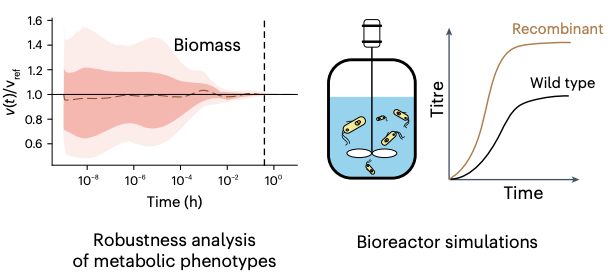
\includegraphics[width=0.5\textwidth]{assets/applications.png}
        \caption{Showcase of usecases of kinematic models. Figure from \cite{rennaissance}.}
        \label{fig:applications}
    \end{figure}

    However, these models require \textbf{thousands} of kinetic parameters, and most of them are \textbf{unknown}, 
    \textbf{hard} to measure, or \textbf{inconsistent} across studies.
    \end{block}

    % ==== Previous Work
    \begin{block}{Previous Work}
        Traditional methods:
        \begin{itemize}
            \item use outdated parameters, rely on brute-force optimization, and assume simplified networks,
            \item struggle with scalability, data uncertainty, and handling multi-scale constraints.
        \end{itemize}
        
        Although attempts have been made to address these issues, they often require:
        \begin{itemize}
            \item \textbf{extensive} computational time \cite{kfit},
            \item \textbf{ground truth training data} derived from traditional kinetic modeling approaches \cite{ischrunk,miskovic2019uncertainty,gans}.
        \end{itemize}
    Finally, newly proposed framework \textbf{RENAISSANCE} \cite{rennaissance} addresses both of these issues,
    however, it still has the following limitations:
    \begin{itemize}
        \item \textbf{unstable convergence} towards finding the optimal kinetic parameters,
        \item requires \textbf{ per environment re-training}.
    \end{itemize}

    \end{block}

\end{column}

% ------ Second column ------
\separatorcolumn
\begin{column}{\colwidth}

    %\vspace{2cm}
    
    \begin{block}{References}
        \nocite{*}
        \small{\bibliographystyle{plain}\bibliography{poster}}
    \end{block}

\end{column}
\separatorcolumn

\end{columns}
\end{frame}
\end{document}